\setcounter{section}{-2}



\section{Preface(前言)}

\subsection{Introduce Myself(自我介绍)}

\frame{
\frametitle{Introduce Myself}
\framesubtitle{自我介绍}
\begin{block}{Name(姓名)}
 BU(布)  Shehui(社辉)
\end{block}
\begin{block}{Office Add.}
 {\Large B3-339} School of computer science and engineering, \\
 South China University of Technology(SCUT), \\
 %Guangzhou higher education mega centre, \\
 %Panyu district, Guangzhou, P.R.China, 510006
\end{block}
\begin{block}{Email}
 $bushehui@scut.edu.cn$ or $bushehui@gmail.com$
\end{block}
\begin{block}{新浪微博}
 $@$布社辉
\end{block}
}

\frame{
\begin{block}{研究方向}
\begin{itemize}
\item Speech prosody(语音韵律),Speech synthesize(语音合成)
\vspace{0.2cm}
\item Speech recognition(语音识别)
\vspace{0.2cm}
\item Speech $\&$ Text Database 
\vspace{0.2cm}
\item Natural language processing(自然语言处理)
\vspace{0.2cm}
%\item Medical imaging technology(超声波医疗诊断成像技术) 
\vspace{0.2cm}
\item Video $\&$ Image Processing
\vspace{0.2cm}
\item Digital Signal Processing
\vspace{0.2cm}
\item $etc.$
\end{itemize}
\end{block}
}



\subsection{Requests of this Course}

\frame{
\begin{center}
\huge{This course is} \\
\vspace{0.2cm}
\Huge{very difficult?}
\vspace{1.5cm}
\begin{block}{}
\Huge{Self$-$learning : Class $\ge$ $3:1$}
\end{block}
\end{center}
}

\frame{
\begin{center}
{\Large Because there are too many contents in the textbook and the course time is limited! \\
$\Downarrow$ \\
Some generial or difficult knowledge will not be introduced in detail.} \\
$\Downarrow$ 
\end{center}
\begin{block}{Requests to you}
\begin{itemize}
\item Please preview the corresponding contents before the lession;
\item Finish the exercises independently and seriously;
\item If you have any questions, please feel free to pick out in the class or contact with me by the email.
\end{itemize}
\end{block}
}

\frame{
\begin{block}{Attendance}
{\Huge Attendance is expected and role will be taken}
\end{block}
\begin{block} {Grading} 
\begin{itemize}
\item 出勤率(Participation) : $10\%$ 
\item 课堂练习(Exercises) : $20\%$  
\item 期末考试(Final exam) :  $70\%$
\end{itemize}
\end{block}
}



\subsection{Introduction of this Course}

\frame{
\begin{center}
\Huge{This course,\\ Why?   \vspace{0.5cm}  \\为什么选择这门课?}
\end{center}
}

\frame{
%\frametitle{Why}
\begin{block}{Three major scientific methods :}
\begin{itemize}
\item Scientific computing $\Rightarrow$ Numerical methods ;
\item Theory;
\item Experiment\footnote{科学计算已和理论、实验并列为三大科学方法。}.
\end{itemize}
\end{block}
\begin{center}
$\Downarrow$
\end{center}
\begin{block}{Numerical Methods :}
\begin{itemize}
\item Solve the mathematics problems by using the computer methods;
\item Involve the mathematical theory;
\item Belong to the applied mathematics\footnote{研究数学计算问题的计算机解决方法和有关数学理论问题的一门学科。属于应用数学的范畴。}.
\end{itemize}
\end{block}
}

\frame{
\begin{center}
\Huge{For example, \\ the computational physics$\ldots$   
\vspace{0.5cm}  
\\例如,计算物理$\ldots$}
\end{center}
}

\frame{
\begin{block}{The computational physics}
\begin{itemize}
\item Based on the computer\footnote{物质基础是计算机;};
\item The key technology is "method" and "programming"\footnote{关键技术是“计算方法”和“程序设计”;}; 
\item The original motivation was the U.S. nuclear weapons development\footnote{原始动力是美国核武器研制的刺激。}.
\end{itemize}
\end{block}
\begin{columns}
\begin{column}{0.3\textwidth}
\begin{center}
"Little boy" and "Hiroshima" in 1945.
\end{center}
\end{column}
\begin{column}{0.7\textwidth}
\begin{figure}
\begin{center}
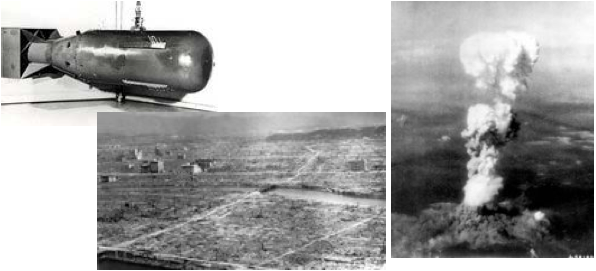
\includegraphics[width=75mm]{chap-0/nuclearbom.png}
\end{center}
\end{figure}
\end{column}
\end{columns}
}

\frame{
\begin{block}{In order to develope nuclear weapons,} 
\begin{itemize}
\item in 1950, only 15 computers worldwide; 
\item to September 1962,  there are 16,187 computers in the U.S. alone\footnote{由于核武器研制需要,1950年全球只有15台计算机,到了1962年9月仅美国就有16187台计算机。}.
\end{itemize}
\end{block}
\begin{figure}
\begin{center}
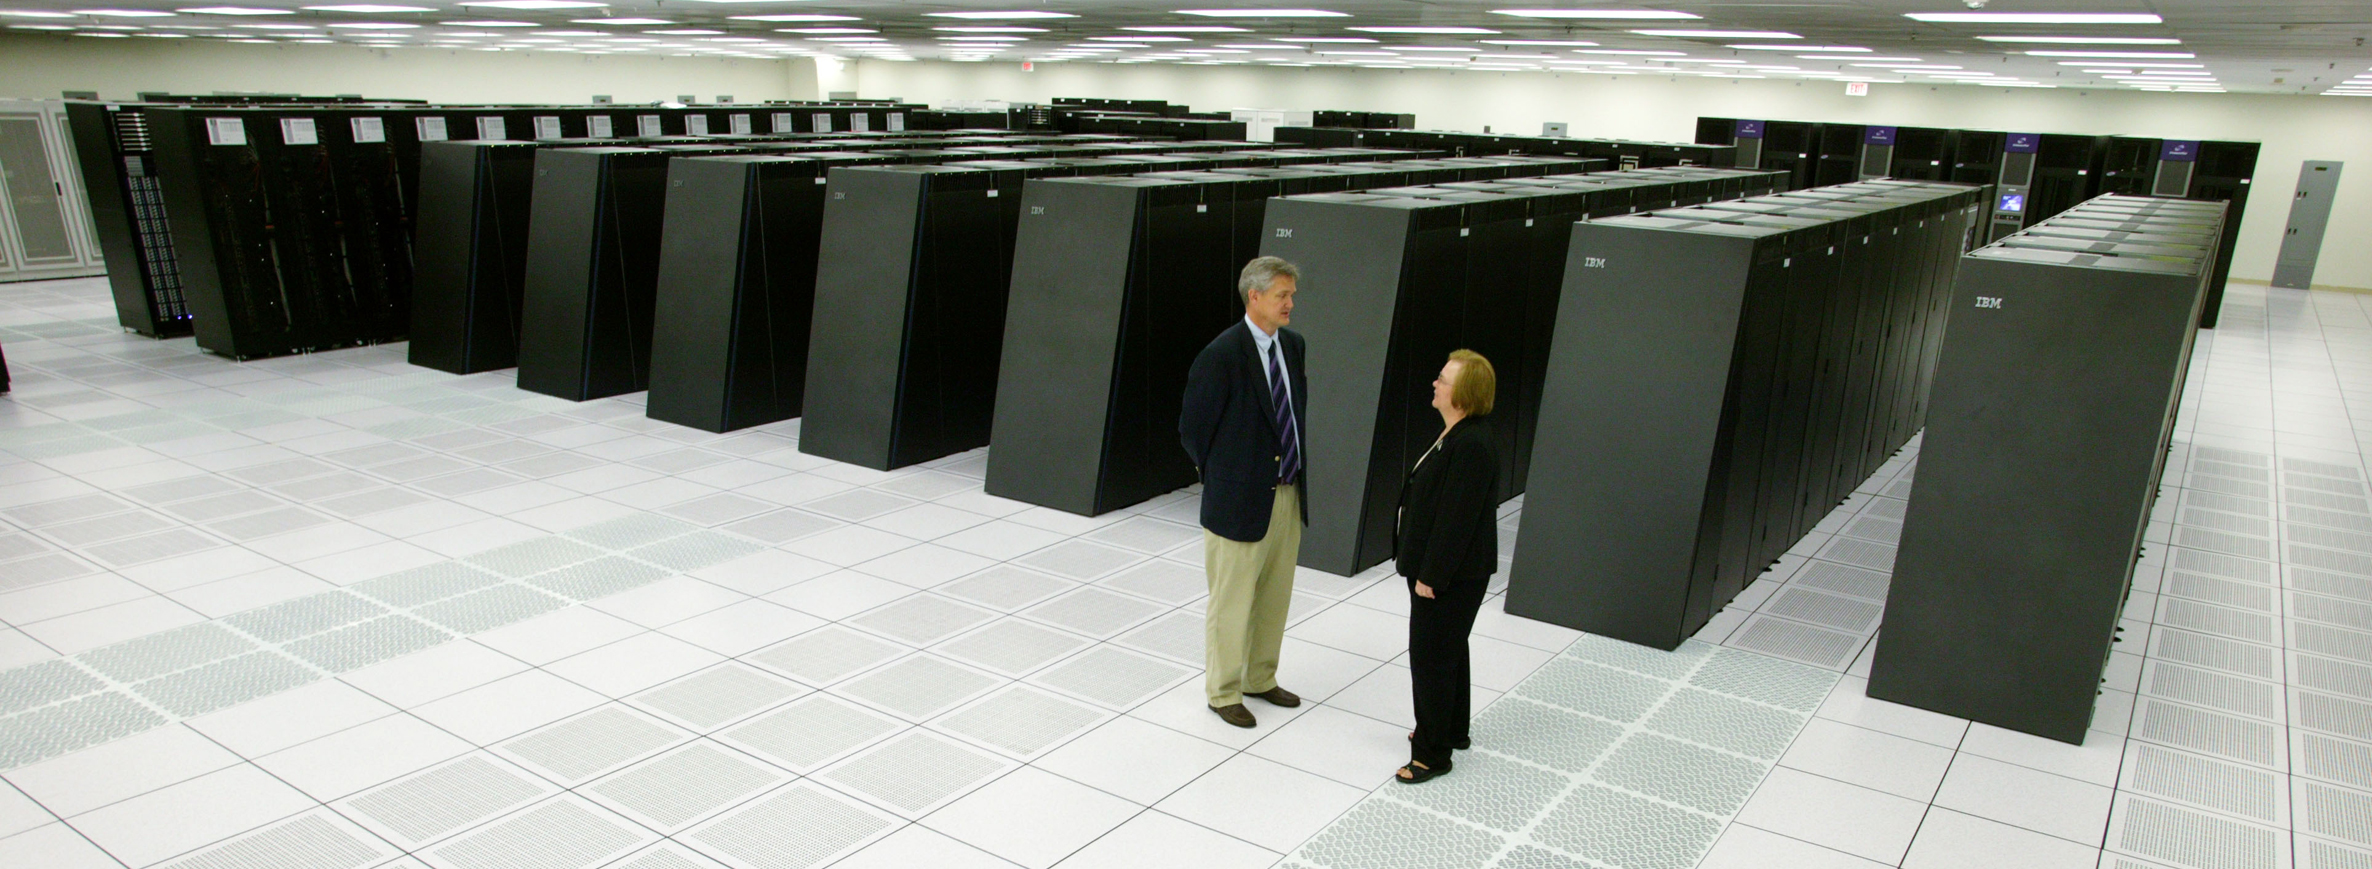
\includegraphics[width=95mm]{chap-0/BlueGene_big.jpg}
\begin{center}
\tiny{Livermore’s BlueGene/L supercomputer}
\end{center}
\end{center}
\end{figure}
}

%\frame{
%\frametitle{Supercomputer}
%\begin{figure}
%\begin{center}
%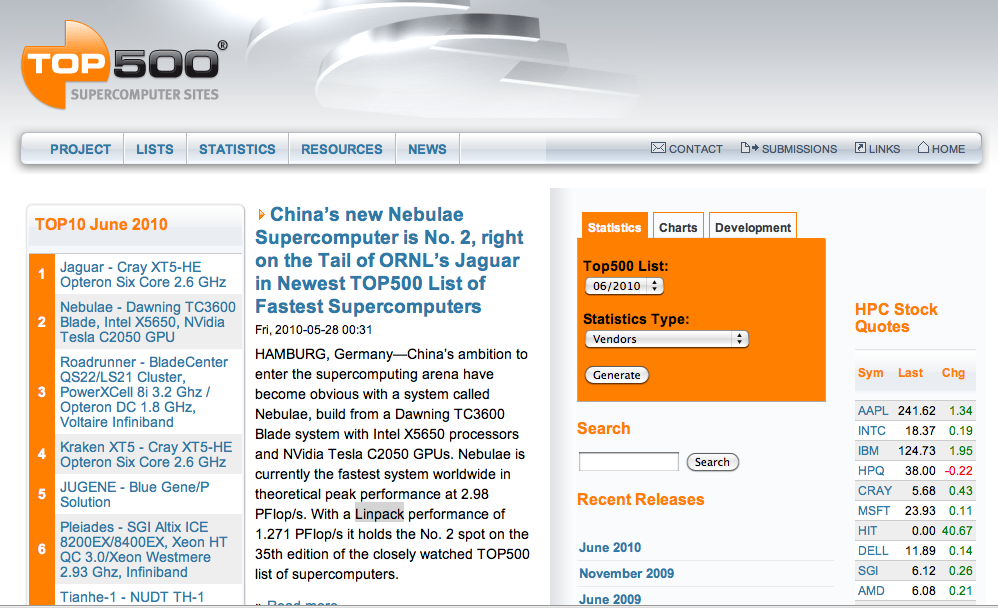
\includegraphics[width=110mm]{chap-0/top500.png} 
%\tiny{\\ Screenshots of "http://www.top500.org/" in Aug. 2010}
%\end{center}
%\end{figure}
%}

%\frame{
%\frametitle{Nebulae Supercomputer}
%\framesubtitle{星云超级计算机}
%\begin{figure}
%\begin{center}
%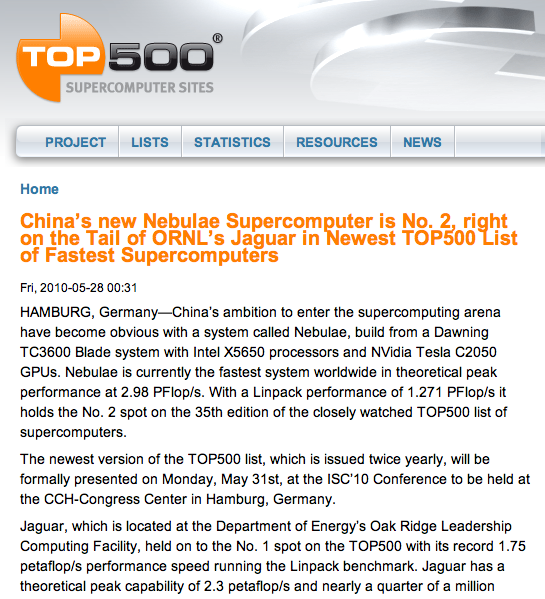
\includegraphics[width=60mm]{chap-0/top500-2.png} 
%\tiny{\\ Screenshots of "http://www.top500.org/lists/2010/06/press-release"}
%\end{center}
%\end{figure}
%}

\frame{
\begin{center}
\huge{
In order to apply the computing power to the solution of practical problems,  \\
the more efficient calculation method must be considered. \\
\vspace{0.2cm}
\begin{block}{}
In other word, \\
The numerical methods is very important\footnote{要把计算机强大的计算能力应用到实际问题的解决上, 必须要有高效的计算方法!}!
\end{block}
}
\end{center}
}

\frame{
\frametitle{Purpose of this Course}
%\framesubtitle{本课程的目的}
\begin{block}{Introduce computer methods for the solution of civil engineering problems, including:}
\begin{itemize}
\item General Introduction to Computer Applications in Engineering and Construction
\item Why do you need to be able to write and understand computer program and numerical methods?
\item Matlab - Mathematical Laboratory
\end{itemize}
\end{block}
\begin{block}{}
\begin{itemize}
\item Enable you to explore in-depth some aspect of Civil, Architectural, or Environmental Engineering of particular interest to you 
\item Provide experience in
\begin{itemize}
\item use of computer methods to solve engineering problems 
\item formulation, execution and presentation of an engineering investigation 
\end{itemize}
\end{itemize}
\end{block}
}

\frame{
\frametitle{Topics of this Course}
\begin{block}{}
\begin{itemize}
\item Fundamental Concepts of Numerical Methods
\begin{itemize}
\item Computer Errors $-$ Recognition and solutions 
\item Linear and Nolinear Algorithm $-$ Setting up multiple sets of equations and solution techniques
\item LU Decomposition (LU分解) $-$ Technique to decompose matrices
\item Eigen-analysis and Eigenvectors $-$ finding the eigenvalues and eigenvectors
\item Interpolation, Polynomial Approximation $\&$ Curve Fitting
\item Numerical Differention $\&$ Integration
\item ODE’s (ordinary differential equations) $-$ Initial Value Problems, Systems of ODE’s of IVP, Boundary Value Problems, Systems of ODE’s of BVP
\item Solution of Differential Equations $\&$ Partial Differential Equations (PDE’s)
\end{itemize}
\item Mathematical Software $\&$ Programming
\begin{itemize}
\item Matlab, Octave, Scilab
%\item C, Java
\end{itemize}
\end{itemize}
\end{block}
}



\frame{
\frametitle{Why do we need to know how to use numerical analysis and methods?}
\begin{block}{You are not going to be given a nice neat exact solution in the “real world”.} 
\begin{itemize}
\item Applications
\item Numerical Errors
\item Computer Types
\item Computer Software
\end{itemize}
\end{block}
}

\frame{
\begin{block}{Applications}
\begin{itemize}
\item Signal Processing
\item CFD (Computational Fluid Dynamics)
\item Structural Analysis
\item Finite Element Analysis
\item Interpolation $-$ Handling data
\item Optimization $-$ Design and estimation
\item CAD (Computer Aided-Drafting) 
\item Data Collection 
\end{itemize}
\end{block}
}

%\frame{
%\begin{block}{Computer  Hardware Types}
%\begin{itemize}
%\item Personal Computer
%\vspace{5mm}
%\item Supercomputers
%\vspace{5mm}
%\item Vector Processors
%\vspace{5mm}
%\item Array Processors
%\vspace{5mm}
%\item Parallel Processor
%\end{itemize}
%\end{block}
%}

%\frame{
%\frametitle{Software}
%\begin{block}{Operating Systems(OS)}
%\begin{itemize}
%\item Windows $-$ Windows XP, Vista, Windows 7
%\item Unix
%\item VMS $-$ VAX
%\item Linux 
%\end{itemize}
%\end{block}
%\begin{block}{Languages}
%\begin{itemize}
%\item Fundamental  Assembler (Bit manipulations)
%\item Engineering Languages
%\begin{itemize}
%\item Fortran, Cobol, Pascal
%\item C++  ( J++ )
%\item Basic
%\end{itemize}
%\item HTML and Java
%\end{itemize}
%\end{block}
%}

%\frame{
%\frametitle{Software}
%\begin{block}{Higher$-$Order Programming}
%\begin{itemize}
%\item Maple $-$ Mathematical Programming Language
%\item Mathematica $-$ Mathematical Programming Language
%\item Java $-$ Internet Programming Language
%\item Matlab $-$ Matrix Laboratory  
%\end{itemize}
%\end{block}
%\begin{block}{Tools}
%\begin{itemize}
%\item Word Processors
%\item Spreadsheets
%\item Database Management
%\item Graphics
%\item Mathematical Computer Codes
%\end{itemize}
%\end{block}
%}

%\frame{
%\begin{block}{What is a program?}
%Program consist of three main components:
%\vspace{0.3cm}
%\begin{itemize}
%\item {\huge Input}
% \vspace{0.3cm}
%\item {\huge Main Program} $-$ Numerical methods and analysis and/or evaluation.
%\vspace{0.3cm}
%\item {\huge Output} $-$ Results.
%\end{itemize} 
%\end{block}
%}

%\frame{
%\begin{block}{Inputs}
%\vspace{0.3cm}
%\begin{itemize}
%\item {\huge Numerical values} 
%\vspace{0.3cm}
%\item {\huge Initialization of the variables}
%\vspace{0.3cm}
%\item {\huge Conditions}
%\vspace{0.3cm}
%\item {\huge Equations}
%\end{itemize}
%\end{block}
%}

%\frame{
%\begin{block}{Main Program }
%Using flow charts, the programs can be designed to perform a task. Using :
%\vspace{0.3cm}
%\begin{itemize}
%\item {\huge Loops}    ($for, do \ldots while$)
%\vspace{0.3cm}
%\item {\huge Conditions} ($if \ldots then \ldots elseif \ldots$, etc$\ldots$ )
%\vspace{0.3cm}
%\item {\huge Error Convergence}  ($while$ )
%\end{itemize}
%\end{block}
%}

%\frame{
%\begin{block}{Outputs .}
% Outputs are the results of the program.  They can go through a series of post-processing methods
%\vspace{0.3cm}
%\begin{itemize}
%\item {\huge Numerical Values}
%\vspace{0.3cm}
%\item {\huge Decisions}
%\vspace{0.3cm}
%\item {\huge Graphs and Plots}
%\end{itemize}
%\end{block}
%}

